\chapter{$n$阶展开方法在微分方程求解中的应用}\label{ch05}
在上一章中, 为了完善齐次平衡原则, 我们提出了$n$阶展开方法, 并将其应用于非线性差分方程的求解. 在这一章中, 我们将以双曲正切方法和\Painleve{}分析为例, 展示$n$阶展开方法在微分方程求解中的应用.

\section{$n$阶展开方法在双曲正切方法中的应用}
和\refchp{ch02}一样, 双曲正切方法的求解对象也是非线性演化方程
\begin{equation}
    U\sbrace{u,u\up{1},u\up{2},\cdots}=0,
\end{equation}
其中, $u=u(x_1,\cdots,x_n)$, 而$U$则是关于$u$及其导数的多项式. 

在双曲正切方法中, 我们首先取行波变换 
\begin{equation}
    \xi = p_1 x_1 +\cdots + p_n x_n + p_{n+1}.  \label{tanh-tw}
\end{equation}
根据链式求导法则, 我们有,
\begin{equation}
    \DIFF{u}{x_k}=\DIFF{u}{\xi}\DIFF{\xi}{x_k}=p_k\DIFF{u}{\xi}.
\end{equation}
基于上述行波变换, 我们可以将原方程转化为关于$u(\xi)$的常微分方程
\begin{equation}
    V(u,u',u'',\cdots)=0. \label{odeq}
\end{equation}

接着, 我们假设\refeqnn{odeq}存在如下形式的解:
\begin{equation}
    u(\xi)=\sum_{k=0}^m{a_k \tanh^k(\xi)}. \label{tanh-poly}
\end{equation}
在原本的双曲正切方法中, 我们基于齐次平衡原则来确定$m$的上界. 现在, 我们可以基于$n$阶展开方法来完善它. 

和\refchp{ch04}一样, 我们用$F(x,m,\mu\up{n})$来表示关于$x$的$m$次$n$阶展开多项式, 其最高$n$项的系数为$\mu\up{n}$. 于是, 我们可以将$u(\xi)$设为
\begin{equation}
    u(\xi)=F\sbrace{\tanh(\xi),m,\alpha\up{n}}.
\end{equation}

由\refeqn{NEM-diff}可知, 要使$u$的关于$\xi$导数也能表示为$n$阶展开多项式, 只需将$\DIF{\xi}\tanh(\xi)$表示为$n$阶展开多项式即可. 我们有 
\begin{equation}
    \DIFF{\tanh(\xi)}{\xi}=1-\tanh^2(\xi)=F\sbrace{\tanh(\xi),2,[-1,0,1]}.
\end{equation}
事实上, \cd{NEPoly}对象已经自动实现了上述转换. 将$u(\xi)$转化为\cd{NEPoly}对象之后, 代入\refeqnn{odeq}, 基于\cd{NEPoly}的微分和乘法操作将\refeqnn{odeq}的所有加法项转化为\cd{NEPoly}列表, 就能调用\cd{nem}求得平衡点的上界$\overline{m}$.

最后, 将$u(\xi)=\sum_{k=0}^{\overline{m}}{a_k \tanh^k(\xi)}$代入\refeqnn{odeq}就能求得原方程的双曲函数解.  此外, 我们在输出时也删除了平凡的解. 按照\refchp{ch03}的做法, 我们也对非平凡的双曲函数解定义了避免取值集合
\begin{equation}
    S=\bbrace{\bbrace{p_k=0}|1\le k \le n} \cup \bbrace{a_1=0,\cdots,a_m=0}.
\end{equation}
式中第一个集合保证解的维数不会退化, 第二个集合保证解不是常数. 

基于上述过程, 我们实现了 NCTM 软件包. NCTM 的核心接口为
\begin{verbatim}
sh:=nctm(eq,a,p,{SP,nExpand});
\end{verbatim}
其中,
\begin{compactitem}[\textbullet]
\item \cd{eq} 是输入的方程.
\item \cd{a} 是\refeqn{tanh-poly}中的待定系数的变量名.
\item \cd{p} 可以是一个变量名, 也可以是一个变量名的列表, 用于指定\refeqn{tanh-tw}中行波变换的系数.
\item 可选参数\cd{SP}表示方程中可以求解的参数. 因为对于一些带参数的方程, 我们有时需要探索方程是否在某些参数条件下有解.
\item 可选参数\cd{nExpand}表示$n$阶展开的阶数, 默认值为2.
\item 返回结果\cd{sh}是一个\cd{SolHolder}对象, 它和TwSolver中的\cd{SolHolder}对象一样, 提供了\cd{get\_sol}\D \cd{verify\_sol}和\cd{plot\_sol}等功能. 
\end{compactitem}

接下来, 我们以几个典型的例子来展示 NCTM 的基本用法, 以及它相对于现有双曲正切函数法的软件包的改进. 

\begin{example}(1+1)Fisher 方程, 用于展示基本用法.

考虑(1+1)Fisher 方程\cite{guo1991analytic},
\begin{equation}
    u_t-u_{x,x}-u(1-u)=0.
\end{equation}
我们取行波变换$\xi=kx+ct+\eta$, 则调用语句为
\begin{verbatim}
sh:=ntcm(eq,a,[k,c,eta]);
\end{verbatim}
最终, NCTM确定$m=2$,
\begin{eqnarray}
    u(\xi)=a_0+a_1 \tanh(\xi)+a_2\tanh^2(\xi).
\end{eqnarray}
同时, \cd{NTCM}给出了4个解
\begin{equation}
    \bbrace{a_0=a_2=\frac{1}{4},a_1=\pm \frac{1}{2},k=\pm \frac{\sqrt 6}{12},c=\frac{5}{6}a_1}. \label{para-rel}
\end{equation}
相比于RATH\cite[p35]{liu2001master}中的两个解, \cd{NTCM}的解更加全面.


\cd{ntcm}函数并没有直接返回解, 需要获取形如\refeqn{para-rel}的参数关系, 则可以调用
\begin{verbatim}
sols:=sh:-get_sols();
\end{verbatim}

如果想要获取解的表达式, 则可以调用\cd{sh:-get\_sol}. 在这个例子中, 调用
\begin{verbatim}
sh:-get_sol(sols[4]);
\end{verbatim}
可以得到
\begin{equation}
    u(x,t)=\frac{1}{4}\sbrace{1+2\tanh\sbrace{\frac{1}{12}(\sqrt{6}x+5t)+\eta}+\tanh^2\sbrace{\frac{1}{12}(\sqrt{6}x+5t)+\eta}}. \label{fisher-sol-4}
\end{equation}

\cd{NTCM}能够保证所得的解是满足关于系数的方程组的. 但是, 如果用户想验证所得的解是否满足原方程, 则可以调用
\begin{verbatim}
sh:-verify_sol(sol);
\end{verbatim}
其中, \cd{sol}是一个参数关系的集合.

最后, 用户还能对所得的解进行绘图. 在这个例子中, 调用
\begin{verbatim}
sh:-plot_sol(sols[4],[x=-10..10,t=-10..20,eta=-2],rest_assign);
\end{verbatim}
可以得到如图\reffig{fisher-tanh}所示的结果. 这是\refeqn{fisher-sol-4}在取$\eta=-2$时的绘图结果. 
    
\end{example}

对于一些带参数的方程, 我们有时需要探索方程是否在某些参数条件下有解. 所以我们将在下一个例子中展示参数\cd{SP}的作用.

\begin{example}允许求解方程参数

对于(1+1)7阶色散方程\cite{duffy1996travelling}
\begin{equation}
    {{u}_{t}}+u\,{{u}_{x}}+p\,{{u}_{3x}}+q\,{{u}_{5x}}+r\,{{u}_{7x}}=0,
\end{equation}
我们设$\xi=kx+ct+\eta$. 若调用
\begin{verbatim}
ntcm(eq,a,[k,c,eta]);
\end{verbatim}
则无解. 此时, 我们允许参数$r$被其它参数表示, 调用
\begin{verbatim}
ntcm(eq,a,[k,c,eta],SP={r});
\end{verbatim}
可以确定$m=6$, 并得到6个解:
\begin{equation}
\def\arraystretch{1.2}
\begin{array}{rl}
r=0:& u=\pm \frac{2\,q\,\sqrt {13}\,c}{\sqrt {-p\,q}}-\frac{3\,{p}^{2}\,\left( 35\,{T}^{4}-70\,{T}^{2}+23\right) }{169\,q},k=-\frac{\sqrt {13}\,\sqrt {-p\,q}}{26\,q};\\
r=\frac{769 q^2}{2500 p}:& u=\frac{1538\,c\,q\,k}{25\,p}+\frac{2250\,{p}^{2}\,\left( 231\,{T}^{6}-693\,{T}^{4}+693\,{T}^{2}-151\right) }{591361\,q},k=\pm \frac{5\,\sqrt {1538}\,\sqrt {-p\,q}}{1538\,q};\\
r=\frac{2519 q^2}{10000 p}:& u=\frac{2159\,c\,q\,k}{25\,p}+\frac{500\,{p}^{2}\,\left( 2079\,{T}^{6}-8316\,{T}^{4}+10395\,{T}^{2}-2738\right) }{4661281\,q},k=\pm\frac{5\,\sqrt {2159}\,\sqrt {-p\,q}}{2159\,q}.\\
\end{array}
\end{equation}
其中, $T=\tanh\sbrace{=kx+ct+\eta}$. 

即使删去$r=0$时的两个解, 我们的解依然比 RATH\cite[p21]{liu2001master} 丰富, 因为RATH只给出了$r=\frac{769 q^2}{2500 p}$和$r=\frac{2519 q^2}{10000 p}$时的两个解.
\end{example}

\begin{figure}[htbp]
\centering
\subfigure[(1+1)Fisher\label{fisher-tanh}]{
    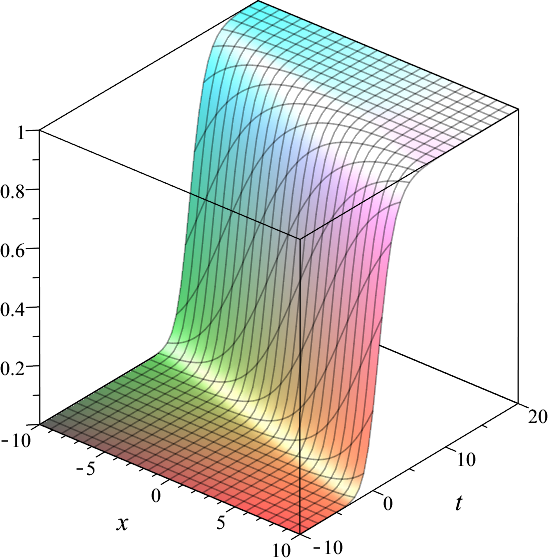
\includegraphics[width=.45\textwidth]{fig/(1+1)Fisher-tanh.png}
}
\subfigure[(2+1)KP\label{kp2-tanh}]{
    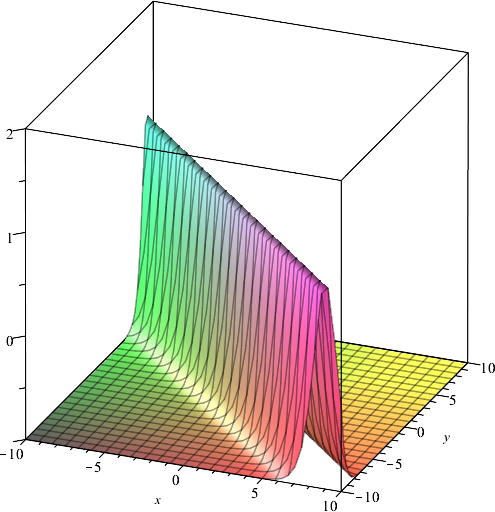
\includegraphics[width=.45\textwidth]{fig/(2+1)KP-tanh.png}
}
\subfigure[(3+1)KP\label{kp3-tanh}]{
    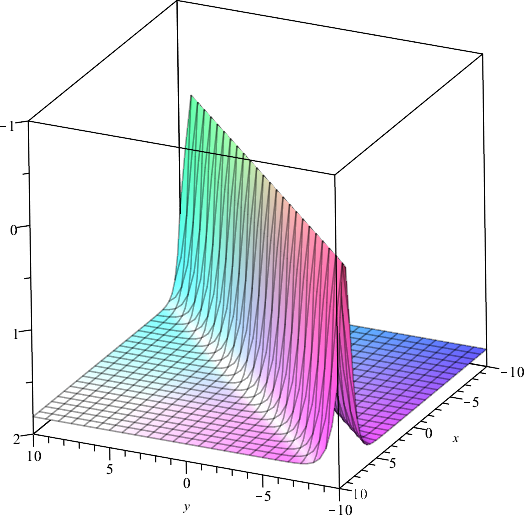
\includegraphics[width=.45\textwidth]{fig/(3+1)KP-tanh.png}
}
\subfigure[(4+1)Fokas\label{fokas-tanh}]{
    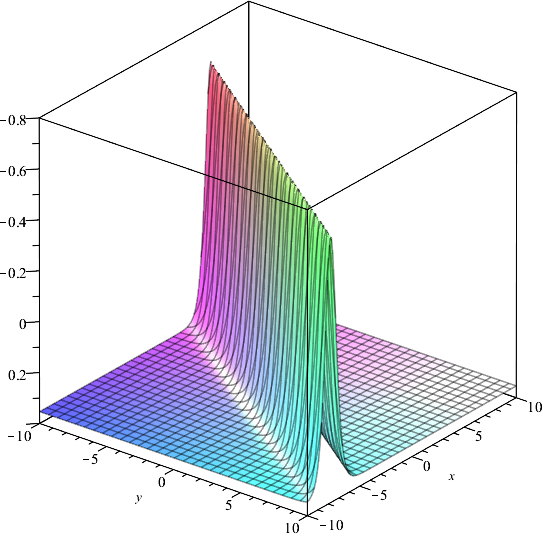
\includegraphics[width=.45\textwidth]{fig/(4+1)Fokas-tanh.png}
}
\caption{一些方程的双曲函数解}
\end{figure}

在以往的双曲正切方法中, 我们主要求解(1+1)维的方程. 而\cd{NTCM}实现了任意维度的行波变换, 所以能够求解更高维度的方程. 现给出几个典型的例子.

\begin{example}(2+1)KP方程\CITEbaKP{}

对于
\begin{equation}
    \alpha\,u_{{{\it yy}}}+6\,uu_{{{\it xx}}}+6\,{u_{{x}}}^{2}+u_{{{\it tx}}}+u_{{{\it xxxx}}}=0,
\end{equation}
我们取$\xi=kx+py+ct+\eta$. \cd{NTCM}确定$m=2$, 并给出了一个解
\begin{equation}
    \left\{ {{a}_{0}}=\frac{\left( 8\,{k}^{4}-\alpha\,{p}^{2}-k\,c\right) }{6\,{k}^{2}},{{a}_{1}}=0,{{a}_{2}}=-2\,{k}^{2}\right\} .
\end{equation}
取$\alpha=k=c=1=\eta=1,t=0$进行绘图, 得到的结果如\reffig{kp2-tanh}所示.
\end{example}

\begin{example}(3+1)KP方程\CITEcaKP{}

对于
\begin{equation}
    -6\,uu_{{{\it xx}}}-6\,{u_{{x}}}^{2}+u_{{{\it tx}}}+u_{{{\it xxxx}}}+3\,u_{{{\it yy}}}+3\,u_{{{\it zz}}}=0,
\end{equation}
我们取$\xi=kx+py+qz+ct+\eta$. \cd{NTCM}确定$m=2$, 并给出了一个解
\begin{equation}
    \left\{ {{a}_{0}}=\frac{\left( -8\,{k}^{4}+k\,c+3\,{p}^{2}+3\,{q}^{2}\right) }{6\,{k}^{2}},{{a}_{1}}=0,{{a}_{2}}=2\,{k}^{2}\right\} .
\end{equation}
取$k=p=q=\eta=1,z=t=0$进行绘图, 得到了如\reffig{kp3-tanh}所示的结果. 
\end{example}

\begin{example}(4+1)Fokas方程\CITEdaFokas{}, 含全部三种平衡点. 

对于
\begin{equation}
    u_{tx}-\frac{1}{4}u_{xxxy}+\frac{1}{4}u_{xyyy}+3u_xu_y+3uu_{xy}-\frac{3}{2}u_{wz}=0 ,
\end{equation}
其次数列表为$\mbrace{2m+2,2m+2,m+4,m+4,m+2}$. 
\begin{compactitem}[\textbullet]
\item 首先, 根据$2m+2=m+4$可以得到第一类平衡点$m=2$.
\item 然后, 考虑$m+4=m+4$, 根据最大性约束有$m+4>2m+2$, 可得$m<2$, 所以有第二类平衡点$m=1$.
\item 最后, 因为有两个$2m+4$, 所以需要考虑第三类平衡点. 我们取$\xi=kx+py+qz+rw+ct+\eta$, 代入后可得$n$阶展开的第一个非零项
\begin{equation}
    \Omega_0 = 24kpa_0^2m\sbrace{m+\frac{1}{2}}. 
\end{equation}
因为$\Omega_0=0$关于$m$没有正整数解, 所以需要$2m+2\le m+4$, 从而得到第三类平衡点的上界为$m=2$.
\end{compactitem}
   
最终, 我们确定确定$m=2$, 这既是第一类平衡点, 也是第三类平衡带点. \cd{NTCM}给出了原方程的两个解
\begin{equation}
    \left\{ k=\pm \sqrt {{p}^{2}+{{a}_{2}}},{{a}_{0}}=-\frac{2\,{{a}_{2}}}{3}-\frac{c}{3\,p}+ \frac{q\,r}{2\,k\,p},{{a}_{1}}=0\right\} .
\end{equation}
取$p=q=r=c=\eta=a_2=1,z=w=t=0$进行绘图, 结果如\reffig{fokas-tanh}所示. 
\end{example}

在之前的例子中, 第三类平衡点并没有起到决定性的作用. 最后, 我们再通过一个只有第三类平衡点的例子来展示\cd{NTCM}中由$n$阶展开方法所带来的优势.

\begin{example}
我们考虑
\begin{equation}
    u(u_t+u_{xxx})+pu_x u_{xx}=0.
\end{equation}
取$\xi=kx+ct+\eta$, 我们调用\verb|ntcm(eq,a,[k,c,eta])|进行求解. 原方程的次数列表为$\mbrace{2m+1,2m+3,2m+3}$, 只存在\BPthree{}. 由
\begin{equation}
    \Omega_0=-{{{a}_{0}}}^{2}\,m\,\left( m\,p+m+2\right) \,\left( m+1\right) \,{k}^{3}
\end{equation}
得到$m=0$. 从而原方程没有非平凡的解. 但是, $m$还有一个可能的零点$m=\frac{-2}{p+1}$. 从而, 当$p$的取值合适时, 原方程可能有任意次数的解. 事实上, \cd{NTCM}对这个情况进行了警告. 

取$p=-3$可以得到$m=1$, 原方程有解 
\begin{equation}
    \left\{ c=-4\,{k}^{3},{{a}_{0}}=0\right\} .
\end{equation}

取$p=-5/4$可以得到$m=8$, 原方程有解 
\begin{equation}
    \left\{ c=16\,{k}^{3},{{a}_{0}}={{a}_{8}},{{a}_{2}}=-4\,{{a}_{8}},{{a}_{4}}=6\,{{a}_{8}},{{a}_{6}}=-4\,{{a}_{8}},a_1=a_3=a_5=a_7=0\right\} .
\end{equation}
\end{example}

\section{$n$阶展开方法在\Painleve{}分析中的应用}
在\Painleve{}分析中, 我们取
\begin{equation}
    u=\sum_{k=1}^{m}\frac{u_k}{f^{m-k+1}}.
\end{equation}
我们可以将其看作是关于$1/f$的多项式
\begin{equation}
    u=F\sbrace{\frac{1}{f},m,\mu\up{n}}.
\end{equation}
在应用$n$阶展开方法时, 因为 
\begin{equation}
    \DIF{x}{\frac{1}{f}}=-\frac{f_x}{f^2}=F\sbrace{\frac{1}{f},2,\mbrace{-f_x,0,0}},
\end{equation}
我们也能根据\refeqn{NEM-diff}完成求导操作. 

在本节中, 我们以一个典型的例子来展示NEM在\Painleve{}分析中的应用.

\begin{example}
考虑方程
\begin{equation}
    u(u_t+u_{xxx})-3u_x u_{xx}=0. \label{pseq}
\end{equation}
其次数列表为$\mbrace{2m+1,2m+3,2m+3}$, 只有\BPthree{}. 由
\begin{equation}
    \Omega_0=2m(m^2-1)u_0^2f_x^3
\end{equation}
可得$m=1$. 将$u=\mu/f$代入原方程后, 关于$1/f$的最高项系数为
\begin{equation}
    3\,\mu\,{{f}_{x}}\,\left( \mu\,{{f}_{xx}}-2\,{{\mu}_{x}}\,{{f}_{x}}\right) .
\end{equation}
可以解得, 
\begin{equation}
    \mu=F(t)\sqrt{f_x}.
\end{equation}
\end{example}
我们取$\mu=\sqrt{f_x}$, 即$u=\sqrt{f_x}/f$代入\refeqnn{pseq}, 可以得到
\begin{equation}
\begin{split}
& 2\,{{f}_{tx}}\,{{{f}_{x}}}^{2}\,f+2\,{{f}_{xxxx}}\,{{{f}_{x}}}^{2}\,f-6\,{{f}_{xx}}\,{{f}_{xxx}}\,{{f}_{x}}\,f+3\,{{{f}_{xx}}}^{3}\,f \\
-&4\,{{{f}_{x}}}^{3}\,{{f}_{t}}-4\,{{f}_{xxx}}\,{{{f}_{x}}}^{3}+6\,{{{f}_{xx}}}^{2}\,{{{f}_{x}}}^{2}=0.
\end{split} \label{pseq-f}
\end{equation}
随后, 我们就能基于\refeqnn{pseq-f}进行各种类型的解的求解.

试试上, 本文所实现的\Painleve{}分析能够自动导出变换$u=F(t)\sqrt{f_x}/f$, 但是我们不能以这个变换为基础进行后续的求解.  因此, 本文实现的 TwSolver 和 NS1L 都不能直接求解\refeqnn{raeq}. 但是, 这两个软件包都提供了自定义变换进行求解的功能.

在TwSolver中, 调用
\begin{verbatim}
twsolve(
    eq,{1},PL=[k,c],
    _utr=(f->sqrt(diff(f,x))/f)
);
\end{verbatim}
就能够指定变换进行求解. 该方程在简单Hirota方法下只有1-孤子解
\begin{equation}
    f=1+\exp\sbrace{k\sbrace{x+\frac{k^2}{2}t}+c}.
\end{equation}
在NS1L中, 也可以利用参数\verb|_utr=(f->sqrt(diff(f,x))/f)|指定变换进行求解. 不过, 该方程没有lump解. 

\section{小结}
在本章中, 我们以双曲正切方法和\Painleve{}分析为例, 展示了$n$阶展开方法在微分方程求解中的作用. 基于NEM实现的双曲正切方法软件包\cd{NTCM}能够求解任意维度的方程, 还能够求解其它双曲正切方法软件包不能求解的方程. 通过\Painleve{}中的一个例子, 也能够看出用$n$阶展开方法替代齐次平衡原则就能求解许多以往不能求解的问题. 

